 % --------------------------------------------------------------
% Copyright Dale Koenig 2018
% --------------------------------------------------------------

%(g;k)--trisection
%update citations

\documentclass[12pt]{amsart}

%\usepackage[margin=1in]{geometry}
\usepackage{amsmath,amsthm,amssymb}
\usepackage{bbm}
\usepackage{mathrsfs}
\usepackage{enumerate}
\usepackage{graphicx}
\usepackage{caption} %%% optional but probably necessary
\usepackage{subcaption} %%% optional but probably necessary
\usepackage{thmtools}
\usepackage{thm-restate}

%\interlinepenalty=300

\newcommand{\N}{\mathbb{N}}
\newcommand{\Z}{\mathbb{Z}}
\newcommand{\R}{\mathbb{R}}
\newcommand{\Q}{\mathbb{Q}}
\newcommand{\C}{\mathbb{C}}
\newcommand{\F}{\mathbb{F}}
\newcommand{\bP}{\mathbb{P}}
\newcommand{\cA}{\mathcal{A}}
\newcommand{\cD}{\mathcal{D}}
\newcommand{\cB}{\mathcal{B}}
\newcommand{\cL}{\mathcal{L}}
\newcommand{\cU}{\mathcal{U}}
\newcommand{\cH}{\mathcal{H}}
\newcommand{\rsS}{\mathscr{S}}
\newcommand{\rsL}{\mathscr{L}}
\newcommand{\rsH}{\mathscr{H}}
\newcommand{\one}{\mathbf{1}}
\newcommand{\del}{\partial }

\newtheorem{thm}{Theorem}
\newtheorem{conj}[thm]{Conjecture}
\newtheorem{prop}[thm]{Proposition}
\newtheorem{claim}[thm]{Claim}
\newtheorem{corr}[thm]{Corollary}
\newtheorem{lemma}[thm]{Lemma}
\theoremstyle{definition}
\newtheorem{ex}[thm]{Example}
\newtheorem{defn}[thm]{Definition}
\newtheorem{question}[thm]{Question}
\theoremstyle{remark}
\newtheorem{rem}[thm]{Remark}
\begin{document}


\title{Trisections of 3--manifold bundles over $S^1$}
\author{Dale Koenig}
\date{}


\begin{abstract}
Let $X$ be a bundle over $S^1$ with fiber a 3--manifold $M$ and with monodromy $\varphi$.
Gay and Kirby showed that if $\varphi$ fixes a genus $g$ Heegaard splitting of $M$ then $X$ has a genus $6g+1$ trisection.
Genus $3g+1$ trisections have been found in certain special cases, such as the case where $\varphi$ is trivial, and it is known that trisections of genus lower than $3g+1$ cannot exist in general.
We generalize these results to prove that there exists a trisection of genus $3g+1$ whenever $\varphi$ fixes a genus $g$ Heegaard surface of $M$.
This means that $\varphi$ can be nontrivial, and can preserve or switch the two handlebodies of the Heegaard splitting.
We additionally describe an algorithm to draw a diagram for such a trisection given a Heegaard diagram for $M$ and a description of $\varphi$.
\end{abstract}

\maketitle

\section{Introduction}
A \emph{trisection} of a closed, smooth, four--dimensional manifold $X$ is a decomposition $X = X_1 \cup X_2 \cup X_3$ such that each $X_i$ is a 4--dimensional handlebody $\natural^{k_i} S^1 \times B^3$ and each pairwise intersection $X_i \cap X_j$, $i \not = j$ is a 3--dimensional handlebody $\natural^g S^1 \times D^2$.
The triple intersection $X_1 \cap X_2 \cap X_3$ is necessarily a closed surface, and by the first two conditions it induces a Heegaard splitting on each $\del X_i$.
Let $g$ denote the genus of the trisection surface $X_1 \cap X_2 \cap X_3$.


Since each $X_i$ is a four--dimensional handlebody $\natural^{k_i} S^1 \times B^3$, $\del X_i$ is diffeomorphic to $\#^{k_i} S^1 \times S^2$.
If $k_1 = k_2 = k_3$ then the trisection is called \emph{balanced} and we say that it is a $(g;k_1)$--trisection of $X$.
Otherwise it is called \emph{unbalanced} and we say that it is a $(g;k_1,k_2,k_3)$--trisection of $X$.
$g$ is called the \emph{genus} of the trisection.
The triple intersection surface, together with three cut systems indicating the boundaries of disks in the three $X_i$ is called a \emph{diagram} of the trisection.
A diagram for a trisection determines the trisection itself up to trisection preserving diffeomorphism.
For more details we refer the reader to the original paper by Gay and Kirby \cite{GayKirby1}.


We also will need to use the notion of (unbalanced) stabilization and destabilization of trisections.
These are described in detail in \cite{MeierSchirmerZupan1}.
Unbalanced stabilization can be performed directly in terms of trisection diagrams.
If $X$ is a trisected 4--manifold, a diagram of the stabilized trisection can be obtained by connect summing a diagram of the original trisection with a genus 1 trisection diagram of $S^4$.
There are three genus 1 trisections of $S^4$ up to diffeomorphism (see Figure \ref{s3g1}), and thus three possible unbalanced stabilizations.
We can similarly view destabilization in terms of diagrams.
Suppose we have a trisection diagram given by surface $\Sigma$ and cut systems $\alpha,\beta,\gamma$.
Suppose there is some simple closed curve $C$ in $\Sigma$ that cuts off a genus 1 trisection diagram of $S^4$.
Then compressing the surface along $C$ and removing the genus 1 diagram for $S^4$ results in a destabilization of the original trisection.


\begin{figure}[h]
\centering
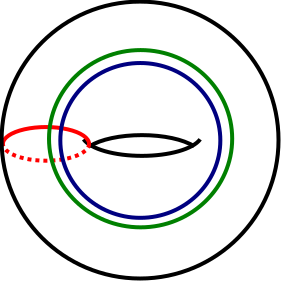
\includegraphics[height=1.6in]{S4trisection_genus1.png}
\caption{One of the three possible genus 1 trisection diagrams of $S^4$ up to diffeomorphism of the diagram surface.
The other two are obtained by recoloring.}
\label{s3g1}
\end{figure}

A \emph{Heegaard splitting} of a closed 3--manifold $M$ is a decomposition of $M$ into two handlebodies intersecting along a surface, called the Heegaard surface.
The \emph{genus} of the splitting is the genus of the surface.
Let $M$ be a smooth 3--manifold with a Heegaard splitting $H_1 \cup_\Sigma H_2$.
Let $\varphi \colon M \to M$ be a self--diffeomorphism of $M$, possibly isotopic to the identity.
We say that $\varphi$ \emph{preserves} the Heegaard splitting if $\varphi(H_1) = H_1$ and $\varphi(H_2)=H_2$.
We say that $\varphi$ \emph{flips} the Heegaard splitting if $\varphi(H_1) = H_2$ and $\varphi(H_2)=H_1$.
In both cases $\varphi(\Sigma) = \Sigma$; that is, $\varphi$ sends the Heegaard surface to itself.
For any choice of $\varphi$, both $H_1 \cup_\Sigma H_2$ and $\varphi(H_1) \cup_{\varphi(\Sigma)} \varphi(H_2)$ are Heegaard splittings of $M$, and if $\Sigma'$ is a stabilization of $\Sigma$ then $\varphi(\Sigma')$ is a stabilization of $\varphi(\Sigma)$.
It follows from the Reidemeister--Singer theorem that after enough stabilizations we get a Heegaard splitting that is preserved by $\varphi$, up to isotopy \cite{Reidemeister1}\cite{Singer1}.


For any 3--manifold $M$ and self--diffeomorphism $\varphi \colon M \to M$ we can construct a 4--manifold by taking $I \times M$ and identifying $(1,x) \sim (0,\varphi(x))$ for all $x \in M$.
For the remainder of the paper, we fix notation to assume that $X$ is always a 4-manifold constructed in this way with $\varphi$ either preserving or flipping a Heegaard splitting $H_1 \cup_\Sigma H_2$ of the fiber $M$.
We henceforth use $g$ to denote the genus of $\Sigma$.
For notational convenience we let $H$ denote an abstract genus $g$ handlebody, so $H$ is in the same diffeomorphism class as both $H_1$ and $H_2$.

In the case where $\varphi$ preserves a genus $g$ Heegaard splitting of $M$, Gay and Kirby showed that $X$ has a $(6g+1;2g+1)$--trisection \cite{GayKirby1}.
In this paper we use similar techniques to improve on this result.
We prove the following:

\begin{thm}
\label{mainresult}
Let $X$ be a bundle over $S^1$ with fiber a closed 3--manifold $M$.
If the monodromy $\varphi$ preserves or flips a genus $g$ Heegaard splitting of $M$, then $X$ has a $(3g+1;g+1)$--trisection.
\end{thm}

We will prove the case where $\varphi$ preserves the splitting and the case where it flips the splitting separately.
Perhaps counterintuitively, the case where $\varphi$ flips the splitting is easier, so we will prove the theorem in this case first.

\begin{rem}
Since we care about how $\varphi$ acts on the Heegaard surface and not just how it acts on $M$, we can have interesting monodromy even when $\varphi$ is isotopic to the identity.
For example, if $H_1$ is isotopic to $H_2$, then $\varphi$ can be isotopic to the identity but still act on $\Sigma$ nontrivially, sending cut systems of $H_1$ to cut systems of $H_2$ and vice-versa.
\end{rem}

After constructing these trisections, we will describe how to construct diagrams for them.
In the case where $\varphi$ flips the Heegaard splitting, we derive the diagram directly.
In the case where $\varphi$ preserves the Heegaard splitting, we will first construct a diagram for a $(4g+1;2g+1,g+1,g+1)$ unbalanced trisection of $X$ and show that we can destabilize down to diagram of the desired $(3g+1;g+1)$ balanced trisection.

There is a correspondence between trisections of a 4--manifold $X$ and certain handle decompositions of $X$.
A trisection can be turned into a handle decomposition of $X$ where $X_1$ corresponds to the 0--handle and 1--handles, $X_2$ to the 2--handles, and $X_3$ to the 3--handles and 4--handle.
Since the rank of the fundamental group cannot be higher than the number of 1--handles in any handle decomposition, $k_1$ gives an upper bound for the rank of $\pi_1(X)$.
By the symmetry of $X_1$, $X_2$, and $X_3$, $k_2$ and $k_3$ give upper bounds for the rank of the fundamental group as well.


Suppose now that $M = \#^g S^1 \times S^2$ and $\varphi$ is trivial.
Then $\varphi$ fixes the standard genus $g$ Heegaard splitting of $M$, so there exists a $(3g+1;g+1)$--trisection of $X$.
The rank of $\pi_1(X)$ is equal to $g+1$ and each $X_i$ is genus $g+1$,  so each $X_i$ is the lowest genus possible.
Since the genera of the $X_i$ together with the Euler characteristic of $X$ determine the genus of the trisection, there exist no trisections of lower genus.
It follows that Theorem \ref{mainresult} cannot be improved in general, although it is possible that there exist lower genus trisections for specific choices of $M$ and $\varphi$.

Much of the work in this paper is covered in the author's doctoral dissertation \cite{koenig1}, which shows that there exists a $(3g+1;g+1)$ trisection when $\varphi$ flips a genus $g$ Heegaard splitting of $M$, or in the case where $\varphi$ is the identity.
In this paper we expand to the case where $\varphi$ is nontrivial but preserves the Heegaard splitting, and provide a more detailed explanation of how to construct diagrams from these trisections.
We will begin in Section \ref{sec_mainthm} by proving Theorem \ref{mainresult}, showing that the proposed trisections exist.
In Section \ref{sec_cutsystems} we will lay the groundwork for analyzing diagrams of these trisections.
In Section \ref{sec_diagrams} we will construct diagrams for the trisections constructed in Section \ref{sec_mainthm}.
Lastly, in Section \ref{sec_questions} we propose some questions for future research.

\subsection*{Acknowledgements} The author would like to give thanks to the anonymous reviewer for giving many useful suggestions, resulting in a much better paper.
The author also gives special thanks to  Jeffrey Meier for his comments on the previous draft of this paper, and to the author's advisor Abigail Thompson for her encouragement and many useful conversations.

%%%%%%%%%%

\section{The Main Theorem}
\label{sec_mainthm}

We split into the two cases.

\smallskip
\noindent\textit{Case 1: $\varphi$ flips the Heegaard splitting}\ \

We view $X$ as being constructed by gluing together the two ends of $I \times M$.
Let $h(x)$ be a self indexing Morse function on $M$ corresponding to the chosen genus $g$ Heegaard splitting of $M$, so $H_1 = h^{-1}([0,3/2])$ and $H_2  = h^{-1}([3/2,3])$.
Define a map $F\colon I \times M \to I \times I$ by $F(t,x) = (t,h(x))$.
We can then cut $I \times I$ into regions as depicted in Figure \ref{flippablebreakdown}, and pull back by $F$ to cut $I \times M$ into regions.
Note that there are two regions labelled $R_2$ and two labelled $R_3$.
The top regions are topological copies of $I \times H_2$ and the bottom regions are copies of $I \times H_1$.
In the following discussion we often refer to regions in $I \times I$ and their pullbacks under $F$ interchangeably.

Since $\varphi$ flips the Heegaard splitting, the left and right side of the rectangle glue together to form a Mobius band.
Hence the two $R_2$ regions are combined into a single contiguous $I \times H$ region, and the two $R_3$ regions are combined into another contiguous $I \times H$ region.
The $R_1$ region is also diffeomorphic to $I \times H$, so this already divides $X$ into three 4 dimensional handlebodies.
However, it is not yet a trisection because the pairwise intersections $R_i \cap R_j$ are not 3 dimensional handlebodies, and in fact are not connected.

\begin{figure}[h]
\centering
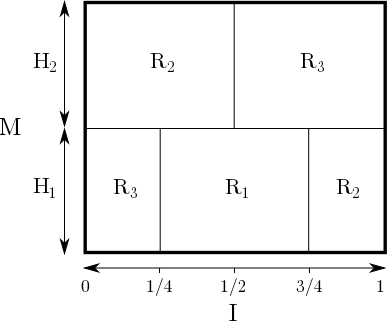
\includegraphics[height=1.8in]{MxS1_flippable.png}
\caption{$I \times I$ is cut into regions as depicted.
Pulling back a vertical slice by the map $F\colon I \times M \to I \times I$ yields a copy of $M$, while pulling back the middle horizontal line yields $I \times \Sigma$.
The vertical $M$ slices are thus cut in half by the middle horizontal line into segments pulling back to $H_1$ and $H_2$, the two halves of the Heegaard splitting.}
\label{flippablebreakdown}
\end{figure}

To fix the pairwise intersections, we make a modification at each horizontal segment in the two dimensional picture lying in some $R_i \cap R_j$.
Note that there are three such segments, since the two segments shown of $R_2 \cap R_3$ are glued together by $\varphi$.
 Let $I_{12} = [1/4,1/2]$, $I_{13} = [1/2,3/4]$, and $I_{23} = [3/4,1] \cup [0,1/4]$, so $I_{ij}$ is the subinterval of $[0,1]$ in which $R_i$ and $R_j$ intersect in a horizontal segment.
The two components of $I_{23}$ are glued together by $\varphi$, so we view it as a single subinterval wrapping around from 1 to 0.
Let $B_{12}$, $B_{23}$, and $B_{13}$ denote three small disjoint balls in $M$, each intersecting the Heegaard surface $\Sigma$ in a single disk.
Let $N_{ij}$ denote $I_{ij} \times B_{ij}$, so $N_{ij}$ is a topological 4--ball.
Define:

\begin{align*}
&X_1 = (R_1 \cup N_{23}) - (\mathring N_{12} \cup \mathring N_{13}) \\
&X_2 = (R_2 \cup N_{13}) - (\mathring N_{12} \cup \mathring N_{23}) \\
&X_3 = (R_3 \cup N_{12}) - (\mathring N_{13} \cup \mathring N_{23})
\end{align*}

Note the similarity to the definition of stabilization of trisections in \cite{GayKirby1}.
$R_1 \cap N_{23}$ consists of two 3--balls, each lying in one component of $\del I_{23} \times B_{23} \subset \del N_{23}$.
Hence $N_{23}$ attaches to $R_1$ as a 1--handle to obtain $X_1$, and since $R_1$ was a 4--dimensional handlebody, $X_1$ is as well.
A similar observation applies to $X_2$ and $X_3$, so each $X_i$ is a genus $g+1$ 4--dimensional handlebody.

We now show that $X_1 \cap X_2$ is a genus $g+1$ handlebody.
The argument for the other two pairwise intersections is identical.
$X_1 \cap X_2$ consists of the following parts:

\begin{itemize}
\item A copy of $I_{12} \times (\Sigma - B_{12})$ coming from the horizontal segment between $R_1$ and $R_2$.
This is the product of an interval and a punctured genus $g$ surface, and is therefore a genus $2g$ handlebody.

\item A copy of $H$ coming from the vertical segment between the $R_1$ and $R_2$ labelled regions.
This is a genus $g$ handlebody.
\item A topological 3--ball $B_a$ coming from $N_{13} \cap X_1$.
\item A topological 3--ball $B_b$ coming from $N_{23} \cap X_2$.
\end{itemize}

$B_a$ intersects each of the $I_{12} \times (\Sigma - B_{12})$ component and the $H$ component of $X_1 \cap X_2$ in a 2--dimensional disk.
The same is true of $B_b$, so both $B_a$ and $B_b$ can be thought of as 3--dimensional 1--handles connecting the $I_{12} \times (\Sigma - B_{12})$ and $H$ components.
$X_1 \cap X_2$ then consists of a genus $2g$ and a genus $g$ handlebody connected by two different 1--handles, resulting in a genus $3g+1$ handlebody.


Since each pairwise intersection is a handlebody and $X_1 \cap X_2 \cap X_3$ is the boundary of each pairwise intersection we have indeed constructed a $(3g+1;g+1)$--trisection of $X$.


\smallskip
\noindent\textit{Case 2: $\varphi$ preserves the Heegaard splitting}\ \

We again begin by cutting up $I \times M$, this time initially cutting it into four regions using Figure \ref{preservebreakdown} as a guide.
Since $\varphi$ preserves the Heegaard splitting, the left and right side of the rectangle glue together to form an annulus.
Define the intervals $I_{13} = [4/5,1] \cup [0,1/5]$, $I_{23a} = [1/5,2/5]$, $I_{24} = [2/5,3/5]$, and $I_{23b} = [3/5,4/5]$.
$R_i$ and $R_j$ intersect in a horizontal segment along $I_{ij}$, and we use $a$ and $b$ to distinguish the two segments where $R_2$ and $R_3$ intersect.
Then the two $R_1$ (resp.
$R_3$) regions are glued together to create a single $R_1$ (resp.
$R_3$) region diffeomorphic to $I \times H$.


\begin{figure}[h]
\centering
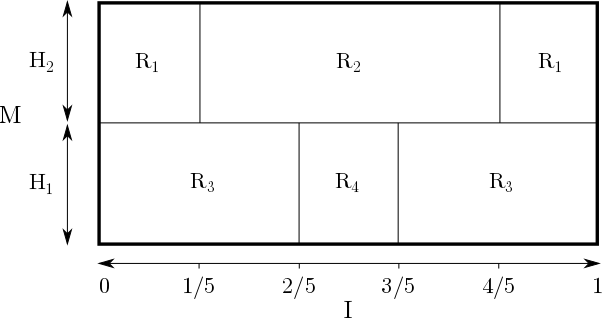
\includegraphics[height=1.8in]{MxS1_preserves.png}
\caption{$I \times M$ is depicted as a rectangle with $I$ as the horizontal axis and $M$ as the vertical axis.
The middle horizontal line represents $I \times \Sigma$, so the copy of $M$ represented by each vertical slice is cut by the middle line into copies of the handlebodies $H_1$ and $H_2$.}
\label{preservebreakdown}
\end{figure}

We further cut up $R_4$ into two smaller regions $R_U$ and $R_V$.
First observe that $R_4 = I_{24} \times H_1$.
Decompose $H_1$ into two three dimensional balls, $U$ and $V$, intersecting in $g+1$ disks as in Figure \ref{fig_disjointballs}.
Then let $R_U = I_{24}  \times U$ and $R_V = I_{24} \times V$.


\begin{figure}[h]
\centering
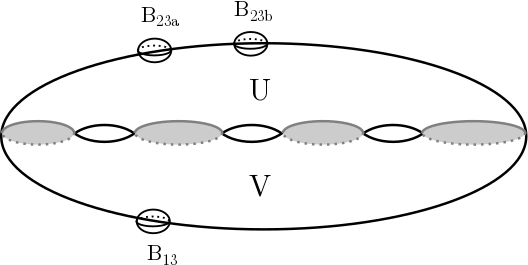
\includegraphics[height=1.6in]{disjointballs.png}
\caption{$H_1$ is decomposed as $U \cup V$ such that $U \cap V$ consists of $g+1$ disjoint disks.
$B_{13}$, $B_{23a}$, and $B_{23b}$ are chosen to be disjoint balls in $H_1 \cup H_2$, each intersecting $\Sigma$ in a disk, such that $B_{23a}$ and $B_{23b}$ intersect $U$.}
\label{fig_disjointballs}
\end{figure}


Now as in the first case choose three small disjoint balls $B_{23a}$, $B_{23b}$ and $B_{13}$ in $M$, each intersecting the Heegaard surface $\Sigma$ in a single disk.
We further require that $B_{23a} \cap H_1$ and $B_{23b} \cap H_1$ lie in $U$ (see Figure \ref{fig_disjointballs}).
Define $N_{23a} = I_{23a} \times B_{23a}$ and define $N_{23b}$ and $N_{13}$ similarly.
Then the trisection is given by:

\begin{align*}
&X_1 = (R_1 \cup R_U \cup N_{23a} \cup N_{23b}) - (\mathring N_{13}) \\
&X_2 = (R_2 \cup N_{13}) - (\mathring N_{23a} \cup \mathring N_{23b}) \\
&X_3 = (R_3 \cup R_V) - (\mathring N_{13} \cup \mathring N_{23a} \cup \mathring N_{23b})
\end{align*}

Each $X_i$ is the union of $I \times H$ with one extra four dimensional 1--handle attaching to $\{0\} \times H$ and $\{1\} \times H$.
This is least clear for $X_1$, where $R_U$, $N_{23a}$, and $N_{23b}$ are each topological four balls, with $R_U$ intersecting each of $N_{23a}$, and $N_{23b}$ in a three dimensional ball.
Thus the union $R_U \cup N_{23a} \cup N_{23b}$ is a 4-ball and it intersects $R_1$ in two three balls, acting as a four dimensional 1--handle.
Similarly, $N_{13}$ intersects $R_2$ in two 3--balls, and $R_V$ intersects $R_3$ in two 3--balls, so they attach as 1--handles.
 We see that each $X_i$ is indeed formed by attaching a single 1--handle to the genus $g$ handlebody $R_i$, and hence is a genus $g+1$ handlebody.
It remains to check that each pairwise intersection is a genus $3g+1$ three dimensional handlebody.
We check this for each pair separately.

$X_1 \cap X_2$ breaks down as follows:

\begin{itemize}
\item Two copies of $H_2$ coming from the two vertical line segments of $R_1 \cap R_2$ in Figure \ref{preservebreakdown}.
Specifically we have $\{1/5\} \times H_2$ and $\{4/5\} \times H_2$.
\item The product $I_{24} \times \Sigma_{0,g+1}$ of an interval and a $g+1$ punctured sphere, coming from the intersection of $R_U$ and $R_2$.
This piece is diffeomorphic to a genus $g$ handlebody.
\item Two topological 3--balls $I_{23a} \times B^2$ and $I_{23b} \times B^2$ coming from $N_{23a} \cap R_2$ and $N_{23b} \cap R_2$.
\item A topological 3--ball $I_{13} \times B^2$ coming from $N_{13} \cap R_1$.
\end{itemize}

Each of the two copies of $H_2$ contributes $g$ to the genus.
$I_{24} \times \Sigma_{0,g+1}$ contributes another $g$ to the genus.
The 3--balls $I_{23a} \times B^2$ and $I_{23b} \times B^2$ each intersect one of the copies of $H_2$ and $I_{24} \times \Sigma_{0,g+1}$ in a disk each, and therefore can be viewed as 1--handles connecting them.
$I_{13} \times B^2$ intersects both copies of $H_2$ in a disk, and therefore can also be viewed as a 1--handle.
It follows that we have three genus $g$ handlebodies which are connected up by the three 1--handles to give a single connected piece.
The union of the genus $g$ handlebodies with $I_{23a} \times B^2$  and $I_{23b} \times B^2$ is a genus $3g$ handlebody, and attaching $I_{13} \times B^2$ adds an additional handle, thus giving a genus $3g+1$ handlebody.

$X_1 \cap X_3$ breaks down as:

\begin{itemize}
\item $I_{13} \times (\Sigma - B_{13})$ coming from the horizontal segment between $R_1$ and $R_3$.
This is the product of an interval and a punctured genus $g$ surface, so it is a genus $2g$ handlebody.

\item A copy of $U$ (a three dimensional ball) lying at each of the two vertical segments between $R_3$ and $R_4$.
\item Two topological 3--balls $I_{23a} \times B^2$ and $I_{23b} \times B^2$ from $N_{23a} \cap R_3$ and $N_{23b} \cap R_3$.
\item $g+1$ copies of $I_{24} \times B^2$ coming from $R_U \cap R_V$.
\end{itemize}


The union of the two copies of $U$ with the $g+1$ copies of $I_{24} \times B^2$ is a genus $g$ 3--dimensional handlebody.
Indeed, each copy of $I_{24} \times B^2$ intersects each copy of $U$ in a single disk, and therefore can be viewed as a 1--handle connecting the two copies of $U$.
The union is then the result of connecting two balls by $g+1$ disjoint 1--handles.
$I_{23a} \times B^2$ and $I_{23b} \times B^2$ each intersect one copy of $U$ in a disk, and $I_{13} \times (\Sigma - B_{13})$ in another disk.
 We then have the a genus $g$ and genus $2g$ handlebody connected by two 1--handles, so the result is then a genus $3g+1$ handlebody.

Lastly, $X_2 \cap X_3$ breaks down as:
\begin{itemize}
\item $I_{23a} \times (\Sigma - B_{23a})$ and $I_{23b} \times (\Sigma - B_{23b})$ coming from the horizontal segments between $R_2$ and $R_3$.
\item A topological 3--ball $I_{13} \times B^2$ coming from $N_{13} \cap R_3$.
\item The product $I_{24} \times \Sigma_{0,g+1}$ of an interval and a $g+1$ punctured sphere, coming from the intersection of $R_V$ and $X_2$.
This piece is diffeomorphic to a genus $g$ handlebody.
\end{itemize}

Note that $\Sigma - B^2$ can be obtained from the $g+1$ punctured sphere by attaching $g$ additional two dimensional 1--handles.
$$\left[ I_{24} \times \Sigma_{0,g+1} \right] \cup \left[ I_{23a} \times (\Sigma - B_{23a}) \right] \cup \left[ I_{23b} \times (\Sigma - B_{23b}) \right]$$ deformation retracts onto $$\left[ I_{24} \times \Sigma_{0,g+1} \right] \cup \left[ \{2/5\} \times (\Sigma - B_{23a}) \right] \cup \left[ \{3/5\} \times (\Sigma - B_{23b}) \right]$$ so it can be built from $I_{24} \times \Sigma_{0,g+1}$ by attaching $g$ 1--handles at each end of $I_{24} \times \Sigma_{0,g+1}$, giving a genus $3g$ handlebody.
The copy of $I_{13} \times B^2$ then adds one more to the genus, for $3g+1$ total.


Since each pairwise intersection is indeed a genus $3g+1$ handlebody, we have successfully constructed a $(3g+1;g+1)$--trisection of $X$.
We constructed genus $3g+1$ trisections in both the cases where $\varphi$ preserves and where it flips the Heegaard splitting, so the main theorem is proven.

%%%%%%%%%
\section{Cut systems, Heegaard diagrams, and Spines}
\label{sec_cutsystems}

The goal of this section is to describe the tools we will use to construct full trisection diagrams in the next section.
After discussing important definitions regarding Heegaard splittings and cut systems, we proceed to show how to construct pieces of trisection diagrams from simple decompositions of $I \times M$.
Extending these methods will allow us to obtain the full trisections in Section \ref{sec_diagrams}.

Let $\Sigma$ be a genus $g$ surface.
A \emph{cut system} for $\Sigma$ is a nonseparating collection of $g$ disjoint curves on $\Sigma$.
Cutting along such a collection results in a $2g$--punctured sphere.
A cut system for $\Sigma$ determines a handlebody $H$ with $\del H = \Sigma$ in the following manner:  First thicken $\Sigma$ to get $[0,1] \times \Sigma$.
Next, for each curve $\alpha$ of the cut system, attach a 2--handle along $\{0\} \times \alpha$.
The result now has two boundary components, one of which is $\{1\} \times \Sigma$ and the other a copy of $S^2$.
Attaching a 3--ball to fill the $S^2$ boundary component gives a handlebody as desired.

Now consider a cut system $\alpha_1,\cdots,\alpha_g$ for $\Sigma$ and let $C$ be a path in $\Sigma$ such that the endpoints of $C$ lie on two different curves $\alpha_i$ and $\alpha_j$ of the cut system.
Assume furthermore that the interior of $C$ is disjoint from the cut system.
$N(\alpha_i \cup \alpha_j \cup C)$ is a thrice punctured sphere with two of its three boundary components parallel to $\alpha_i$ and $\alpha_j$ respectively.
Replacing $\alpha_i$ with the third boundary component gives a new cut system.
Such a move is called a \emph{slide} of $\alpha_i$ over $\alpha_j$.
Two cut systems are called \emph{slide equivalent} if there is a sequence of slides relating them.
Two cut systems are slide equivalent if and only if they determine the same handlebody \cite{Johannson1}.
Two collections of cut systems $\delta_1,\cdots,\delta_m$ and $\delta_1',\cdots,\delta_m'$ are called \emph{slide--diffeomorphic} if there is a diffeomorphism $\phi\colon \Sigma \to \Sigma$ such that each $\phi(\delta_i)$ is slide equivalent to $\delta_i '$.
The two relevent cases are $m=2$ (slide-diffeomorphic Heegaard diagrams) and $m=3$ (slide-diffeomorphic trisection diagrams).

Given a Heegaard splitting $M = H_1 \cup H_2$, a \emph{Heegaard diagram} $(\Sigma; \alpha, \beta)$ consists of the surface $\Sigma$ together with cut systems $\alpha_1,\cdots,\alpha_g$ and $\beta_1,\cdots,\beta_g$ determining $H_1$ and $H_2$ respectively.
By the above remarks, slide--diffeomorphic Heegaard diagrams give diffeomorphic 3--manifolds, and in fact that diffeomorphism can be chosen to preserve the Heegaard splitting.
When drawing a Heegaard surface, the surface can always be embedded in $\R^3$ such that it is a restriction of an embedding of $H_1$ into $\R^3$.
Thus, a standard system of meridians corresponds to a cut system for $H_1$.
In figures we always choose embeddings of this sort, so the curves bounding disks in $H_1$ are precisely the curves that ``look like" they bound disks.

We can now analyze how to obtain cut systems from the regions $R_i$ in the previous section.
Let $M = H_1 \cup H_2$ be a 3--manifold with a Heegaard splitting.
Consider the rectangular regions shown in in Figure \ref{sectionbreakdown}.
Recall that this rectangle is the image of a map $F\colon I \times M \to I \times I$, where $F(t,x) = (t,h(x))$ with $h\colon M \to I$ a self indexing Morse function on $M$.
We see two vertical line segments in Figure \ref{sectionbreakdown}, the vertical components of $R_1 \cap R_3$ and of $R_2 \cap R_3$.
Pulling back the left vertical line segment by $F$ corresponds to a copy of $H_1$ and pulling back the right to a copy of $H_2$.
We will work through this example in depth, and then comment on how to extend to other cases.


\begin{figure}[h]
\centering
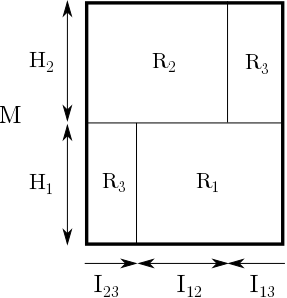
\includegraphics[height=1.8in]{MxS1_section.png}
\caption{We analyze the part of the spine and trisection surface lying in the region shown.}
\label{sectionbreakdown}
\end{figure}

In constructing (a restriction of) a trisection from Figure \ref{sectionbreakdown}, we first choose small disjoint balls $B_{12}$, $B_{13}$, $B_{23}$ in $M$, each intersecting $\Sigma$ in a disk.
Letting $N_{13} = I_{13} \times B_{13}$, $N_{12} = I_{12} \times B_{12}$, and $N_{23} = I_{23} \times B_{23}$ to $X_1$, we can define

\begin{align*}
&X_1 = (R_1 \cup N_{23}) - (\mathring N_{12} \cup \mathring N_{13}) \\
&X_2 = (R_2 \cup N_{13}) - (\mathring N_{12} \cup \mathring N_{23}) \\
&X_3 = (R_3 \cup N_{12}) - (\mathring N_{13} \cup \mathring N_{23})
\end{align*}

Let us analyze how the trisection surface $X_1 \cap X_2 \cap X_3$ intersects the pull back of each vertical cross section.
Let $M_t = \{t\} \times M$ denote the pullback $F^{-1}(\{t\} \times I)$.
If $t$ lies in the interior of $I_{23}$, then $M_t \cap X_1$ is the 3--ball $B_{23}$.
$\del B_{23}$ decomposes into two disks, one intersecting $R_2$ and one intersecting $R_3$.
The meridian circle $\del B_{23} \cap \Sigma$ lies in the triple intersection.
Similarly if $t$ lies in the interior of $I_{12}$ then $M_t \cap (X_1 \cap X_2 \cap X_3) = \del B_{12} \cap \Sigma$, which is homeomorphic to $S^1$.
If it lies in the interior of $I_{13}$ it is the circle $\del B_{13} \cap \Sigma$.
Thus in the interior $\mathring I_{ij} \times M$ of each $I_{ij} \times M$ region the triple intersection is the open cylinder $\bigcup_{x \in \mathring I_{ij}} S^1$.


The intersection $R_1 \cap R_2 \cap R_3$ consists of two points in the figure, which pull back under $F$ to two copies of $\Sigma$.
We call the pullback of the left point $\Sigma_1$ and the pullback of the right point $\Sigma_2$.
After adding the tubes $N_{ij}$, $\Sigma_1$ has punctures $B_{23} \cap \Sigma_1$ and $B_{12} \cap \Sigma_1$, while $\Sigma_2$ has punctures $B_{13} \cap \Sigma_2$ and $B_{12} \cap \Sigma_2$.
The $B_{12} \cap \Sigma_i$ punctures of the two surfaces are connected by the open tube in $I_{12} \times M$.
 The part of the triple intersection lying in the pullback of the figure therefore is a twice punctured genus-$2g$ surface as seen in Figure \ref{fig_coresubsurface}.
When drawing $\Sigma_1$ and $\Sigma_2$, we embed into $\R^3$ such that obvious meridians correspond to curves bounding disks in $H_1$.
That is, if we view the surface as the boundary, minus some disks, of a standardly embedded handlebody in $\R^3$, then a simple closed curve bounds a disk in that handlebody if and only if it bounds a disk in $H_1$ when considered to be a (punctured) Heegaard surface for $M$.
Additionally, we choose the embedding so that the orientation induced by $H_1$ on each $\Sigma_i$ is the same as the orientation induced by the handlebody it bounds in the embedding into $\R^3$.
This forces the drawn portion of the trisection surface to be immersed rather than embedded, as the tube connecting $\Sigma_1$ and $\Sigma_2$ must pass through one of the copies of $\Sigma_i$ as depicted in Figure \ref{fig_coresubsurface}.
After determining cut systems bounding curves in each $X_i \cap X_j$, we will remap the surface into $\R^3$ to get an embedding.

\begin{figure}[h]
\centering
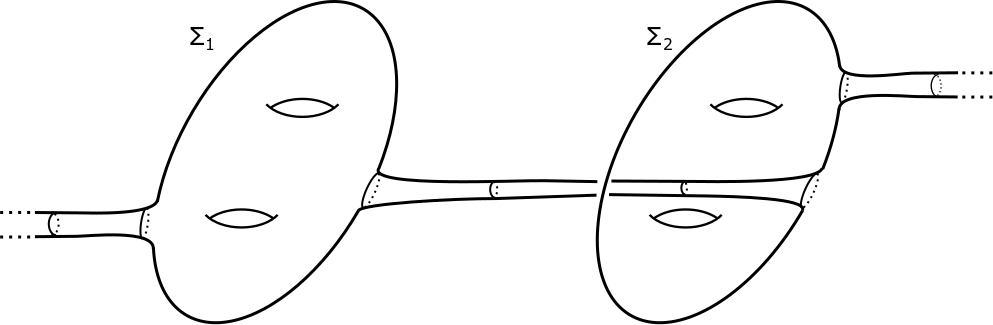
\includegraphics[height=1.6in]{coresubsurface.png}
\caption{A restricted section of the trisection surface.}
\label{fig_coresubsurface}
\end{figure}

We can now begin constructing the trisection diagram.
Let $\{\alpha_i\}_{1 \le i \le n}$ be a cut system for $X_1 \cap X_2$, $\{\beta_i\}_{1 \le i \le n}$ for $X_1 \cap X_3$, and $\{\gamma_i\}_{1 \le i \le n}$ for $X_2 \cap X_3$.
Since $\Sigma_1$ bounds $H_1$ in $X_1 \cap X_3$, we can draw a cut system for $H_1$ on it as $\beta$ curves.
Similarly, since $\Sigma_2$ bounds $H_2$ in $X_2 \cap X_3$, we can draw a cut system for $H_2$ on it as $\gamma$ curves.
A meridian of the tube connecting the two copies of $\Sigma$ corresponds to a meridian of the 2--sphere $\del B_{12}$.
This meridian cuts $\del B_{12}$ into a disk lying in $X_2 \cap X_3$ and a disk lying in $X_1 \cap X_3$, so we can draw both a $\beta$ and $\gamma$ curve on it.
Similarly, we can draw an $\alpha$ and $\beta$ curve as meridians of the tube leaving the left side of the picture, and an $\alpha$ and $\gamma$ curve as meridians of the tube leaving the right side of the picture.
Note however that there is some redundancy here --- drawing all of the curves mentioned will separate the surface, so in fact only one of the tube meridians needs to be marked for each of the three cut systems.

When drawing the cut systems on $\Sigma_1$ and $\Sigma_2$ we did not specify how the curves lie with respect to the punctures.
It turns out, however, that the location of the punctures does not matter.
Indeed, sliding the puncture over some curve of the cut system corresponds to sliding the curve of the cut system over the meridian curve of the tube.
For example, sliding the leftmost puncture over one of the meridian $\beta$ curves on $\Sigma_1$ corresponds to a slide of that $\beta$ curve over the $\beta$ curve that is a meridian of the tube.
Hence, the location of the punctures on a copy of $\Sigma$ with respect to the curves drawn on $\Sigma$ does not matter.
However, we require that the two punctures on the two copies of $\Sigma$ connected by the tube are in the same place on their respective copy of $\Sigma$.


It remains to draw the $\alpha$ curves bounding disks in the $I_{12} \times (\Sigma - B_{12} \cap \Sigma)$ section of $X_1 \cap X_2$.
 Let $c$ be an arc in $\Sigma$ with interior disjoint from the three $B_{ij} \cap \Sigma$ disks, and endpoints lying on the puncture $\del B_{12} \cap \Sigma$.
$I_{12} \times c$ is then a topological disk lying in $I_{12} \times (\Sigma - B_{12} \cap \Sigma)$.
The boundary of the disk consists of a copy of $c$ in each of $\Sigma_1$ and $\Sigma_2$ and the pair of arcs $I_{12} \times \del c$ connecting them.
This is true regardless of the choice of $c$, so in fact choosing a nonseparating collection of $2g$ such arcs in $\Sigma - B_{12} \cap \Sigma$ will result in $2g$ such $\alpha$ curves.
The result after drawing one such curve is shown in Figure \ref{fig_coresubsurfacediagram}.
The figure uses the simplest case of $M = S^3$, so the $\gamma$ curve cut system for $H_2$ consists of longitude curves.
In this and future diagrams, $\alpha$ curves are drawn in red, $\beta$ in blue, and $\gamma$ in green, easily remembered since (b)eta curves are (b)lue and (g)amma curves (g)reen.

\begin{figure}[h]
\centering
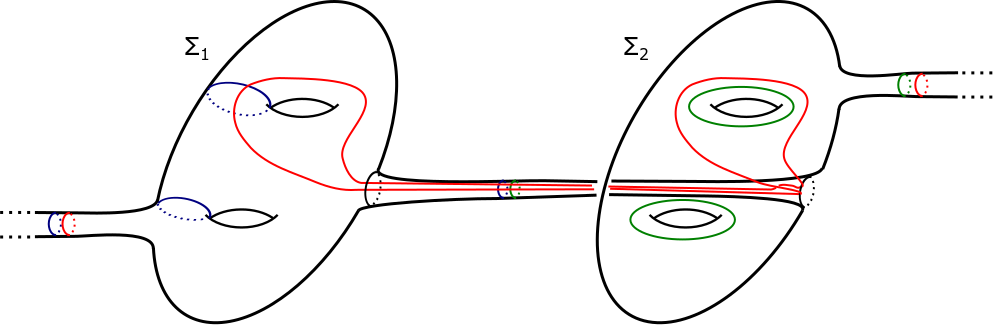
\includegraphics[height=1.6in]{coresubsurfacediagram.png}
\caption{The arc $c$ is chosen to loop once around the top hole of $\Sigma$.
Slices of the disk $I_{12} \times c$ are shown as dotted curves, with the boundary giving the new $\alpha$ curve.}
\label{fig_coresubsurfacediagram}
\end{figure}

Lastly we want to remap the diagram into $\R^3$ to get an embedding.
We do this by reflecting one of the two copies of $\Sigma$ across the vertical axis in the page.
This reflection replaces the cut system for $H_1$ or $H_2$ on that copy of $\Sigma$ with its reflection.
After this reflection, the $\alpha$ curves passing through the middle tube are symmetric across the tube, and the tube can be homotoped to an embedding.
The resulting partial diagram obtained from reflecting $\Sigma_2$ in Figure \ref{fig_coresubsurfacediagram} is shown in Figure \ref{fig_coresubsurfacediagram_embedded}.

\begin{figure}[h]
\centering
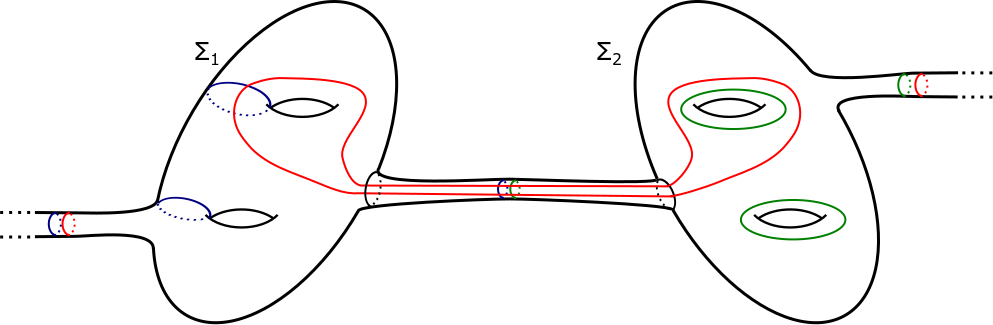
\includegraphics[height=1.6in]{coresubsurfacediagram_embedded.png}
\caption{The result of remapping so that the surface is embedded.
The $\alpha$ curve passing through the tube is now symmetric.
The diagram could be completed by extending to a nonseparating collection of four disjoint symmetric $\alpha$ curves.}
\label{fig_coresubsurfacediagram_embedded}
\end{figure}

We now comment on the other possible cases.
In Figure \ref{sectionbreakdown}, the left vertical line segment pulls back under $F$ to a copy of $H_1$ in the spine, while the right pulls back to a copy of $H_2$.
The resulting trisection diagram therefore has a cut system for $H_1$ on $\Sigma_1$, and a (reflected) cut system for $H_2$ on $\Sigma_2$.
The same method works as long as the cut systems are chosen to match with the vertical line segment.
If the left vertical line segment corresponds to $H_2$, we draw a cut system for $H_2$ on $\Sigma_1$.
Similarly if the right vertical segment corresponds to $H_1$, we draw a reflected cut system for $H_1$ on $\Sigma_2$.
Lastly, shuffling the indices of the regions $R_i$ will recolor the curves, switching $\alpha$, $\beta$, and $\gamma$ curves, but will not change curves of the diagram themselves.

%%%%%%%%%
\section{Constructing the trisection diagrams}
\label{sec_diagrams}

Again we split into the two separate cases.
We proceed from the previous descriptions of the trisections, finding cut systems for each of the three pairwise intersections $X_i \cap X_j$.
As before, it is easier to start with the case where $\varphi$ flips the Heegaard splitting.

\smallskip
\noindent\textit{Case 1: $\varphi$ flips the Heegaard splitting}\ \

We begin by recalling the form of triple intersection surface.
Each triple intersection corner in Figure \ref{flippablebreakdown} gives a twice punctured copy of $\Sigma$, and the horizontal segments connecting two corners give tubes connecting the appropriate copies of $\Sigma$.
The trisection surface $X_1 \cap X_2 \cap X_3$ then consists of three copies of $\Sigma$ connected by three tubes.
This results in a genus $3g+1$ surface.
We construct the diagram keeping this in mind, drawing three copies of $\Sigma$ and connecting them with tubes.


Let $\Sigma_1$, $\Sigma_2$, and $\Sigma_3$ be the (twice punctured) copies of $\Sigma$ lying at the three triple intersection corners from left to right.
So $\Sigma_1$ is a twice punctured Heegaard surface of $M_{1/4}$, $\Sigma_2$ of $M_{1/2}$, and $\Sigma_3$ of $M_{3/4}$.
The product $[1/4, 3/4] \times M$ induces a natural identification between $M_{1/4}$, $M_{1/2}$, and $M_{3/4}$, and restricting to $\Sigma$ gives a natural identification between the three $\Sigma_i$.
We denote these identifications as $\eta_{1 \to 2}\colon \Sigma_1 \to \Sigma_2$, $\eta_{1 \to 3}\colon \Sigma_1 \to \Sigma_3$, and $\eta_{2 \to 3}\colon \Sigma_2 \to \Sigma_3$.
$I_{23} \times M$ induces a different identification $\eta_{3 \to 1}$ between $M_{3/4}$ and $M_{1/4}$, and this also restricts to give an identification of $\Sigma_3$ and $\Sigma_1$.
The composition $(\eta_{1 \to 3} \circ \eta_{3 \to 1})$ is the identification $\Sigma_3 \to \Sigma_3$ given by going once around the base $S_1$ of the fiber bundle, which is precisely $\varphi$.
Thus, we find that $\eta_{3 \to 1} = (\eta_{1 \to 3}^{-1} \circ \varphi)$.
That is, to see how a curve or arc in $\Sigma_3$ gets mapped to $\Sigma_1$ by pushing it through $I_{23} \times \Sigma$, first apply $\varphi$ to it and then use the identification $\eta_{1 \to 3}^{-1}$ to bring it to $\Sigma_1$.

We can see now that the location that the punctures are drawn is not completely free.  Indeed, for any two punctures that are tubed together, drawing one of the two determines where we must draw the other.  So for example the punctures of $\Sigma_1$ and $\Sigma_2$ that are tubed together should be drawn so that they are identified by $\eta_{1 \to 2}$.  Now that $\eta_{1 \to 3}$ has been described, we can apply this to the punctures of $\Sigma_1$ and $\Sigma_3$ that are tubed together as well.

Embed $\Sigma_1$, $\Sigma_2$ and $\Sigma_3$ into $\R^3$ along three axes $\theta_1,\theta_2$, $\theta_3$ evenly distributed in $\theta$ as in Figure \ref{embeddingsigmas}.
We embed such that that rotating $\Sigma_1$ by $2\pi/3$ and then reflecting induces $\eta_{1 \to 2}$.
Similarly rotating $\Sigma_1$ by $4\pi/3$ (with no reflection) induces $\eta_{1 \to 3}$.
We choose the embedding of $\Sigma_1$ so that a cut system of $H_1$ coincides with an obvious system of meridians, and the simple nature of $\eta_{1 \to 2}$ and $\eta_{1 \to 3}$ ensures that this is true for our embeddings of $\Sigma_2$ and $\Sigma_3$ as well.
For $\Sigma_1$ and $\Sigma_3$, we require that the orientation induced by $H_1$ is the same as the orientation induced by the handlebodies they bound in $\R^3$.
For $\Sigma_2$, the orientation induced by $H_1$ is opposite the orientation induced by the handlebody bounded in $\R^3$.

\begin{figure}[h]
\centering
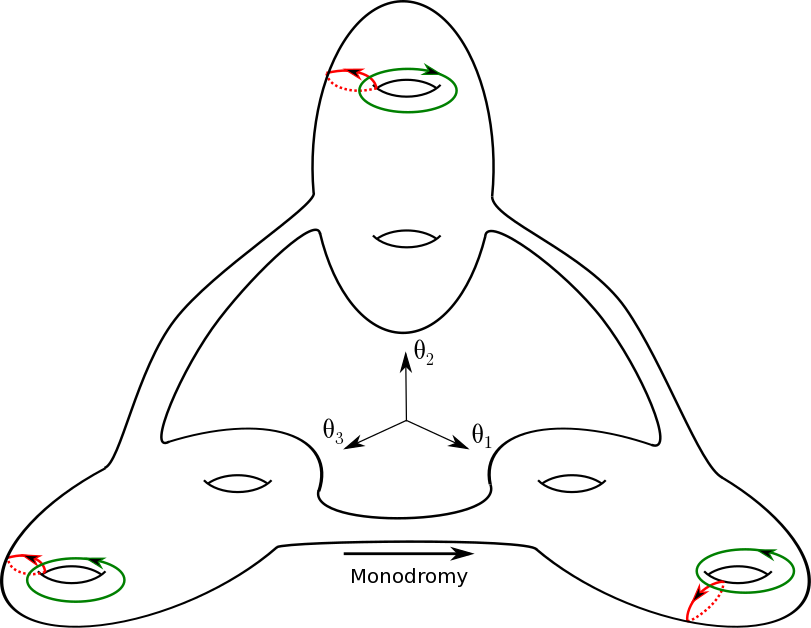
\includegraphics[height=3in]{sigmas.png}
\caption{  The top copy of $\Sigma$ has been reflected about $\theta_2$.
The orange and purple oriented curves in each copy of $\Sigma$ therefore are the same pair of curves slid along $I \times \Sigma$.
Passing through the gluing monodromy, however, will send orange and purple curve to something else in general.}
\label{embeddingsigmas}
\end{figure}

With this setup, we can use the discussion of Section \ref{sec_cutsystems} to draw the curves of the trisection diagram.
On each $\Sigma_i$ either a copy of $H_1$ or of $H_2$ lies in the spine with boundary $\Sigma_i$, so we draw the appropriate cut system.
On $\Sigma_2$, the cut system is reflected to match the embedding.
One curve from each $\alpha$, $\beta$, and $\gamma$ cut system is drawn as a meridian of one of the tubes connecting two $\Sigma_i$, and symmetric curves bounding disks in $I \times (\Sigma - D^2)$ are drawn crossing the tubes.
The construction differs from the discussion of Section \ref{sec_cutsystems} only in the region $I_{23} \times (\Sigma - D^2)$.
The curves drawn here will not in general be symmetric.
Given an arc $c \in \Sigma_3$ with boundary lying on $\Sigma_3 \cap \del B_{13}$, the disk $I_{23} \times c$ lies in $X_1 \cap X_3$, so its boundary is a $\gamma$ curve.
The boundary of the disk $I_{23} \times c$ consists of $c \subset \Sigma_3$, $\eta_{3 \to 1}(c) \subset \Sigma_1$, and two arcs in the tube between $\Sigma_1$ and $\Sigma_3$ connecting the corresponding ends of $c$ and $\eta_{3 \to 1}(c)$.


We can now describe the algorithm to draw the trisection diagram.
Let $\theta_1$, $\theta_2$, and $\theta_3$ be three angles equidistributed in $S^1$ as before.
Let $\theta_{ij}$ denote the angle halfway between $\theta_i$ and $\theta_j$, lying in the smaller ($<\pi$) angular region between them.
We describe $\alpha$ curves determining a cut system for $X_1 \cap X_2$, $\beta$ curves a cut system for $X_1 \cap X_3$, and $\gamma$ curves a cut system for $X_2 \cap X_3$.

\begin{enumerate}
\item Draw the genus $3g+1$ surface as three twice punctured copies $\Sigma$ with tubes connecting each pair.
Denote the copies of $\Sigma$ by $\Sigma_1$, $\Sigma_2$, and $\Sigma_3$, lying at $\theta_1$, $\theta_2$, and $\theta_3$ respectively.
\item Draw $2g$ nonseparating disjoint $\alpha$ curves symmetric about $\theta_{12}$ and $2g$ nonseparating disjoint $\beta$ curves symmetric about $\theta_{23}$.
The $\alpha$ curves necessarily avoid $\Sigma_3$ and similarly the $\beta$ curves necessarily avoid $\Sigma_1$.
These are the curves bounding product disks in $I_{12} \times (\Sigma - D^2)$ and $I_{13} \times (\Sigma - D^2)$ respectively.
\item Draw a cut system for $H_1$ on $\Sigma_1$ as $\beta$ curves and on $\Sigma_3$ as $\alpha$ curves.
\item Draw a parallel $\alpha$ and $\beta$ curve as meridians of the tube connecting  $\Sigma_1$ and $\Sigma_3$ (so at $\theta_{23}$).

\item On $\Sigma_2$ draw a cut system for $H_2$ as $\gamma$ curves.
The cut system should be reflected about $\theta_2$ to match the embedding of $\Sigma_2$.
\item Draw a $\gamma$ curve as a meridian of the tube connecting $\Sigma_2$ with either $\Sigma_1$ or $\Sigma_3$.
The two choices are slide equivalent.
\item Let $c_1,\cdots,c_{2g}$ be a nonseparating collection of disjoint arcs in $\Sigma_3$ with their boundaries lying on the puncture $\{3/4\} \times \del B_{23} \subset \Sigma_3$ that is tubed to the puncture $\{1/4\} \times \del B_{23} \subset \Sigma_1$.
Recall that these two punctures are identified by $\eta_{3 \to 1}$.
Then $\eta_{3 \to 1}(c_1),\cdots,\eta_{3 \to 1}(c_{2g})$ is a nonseparating collection of disjoint arcs in $\Sigma_1$ with their boundaries lying on the puncture of $\Sigma_1$ that is tubed to $\Sigma_3$.
Draw $2g$ nonseparating disjoint $\gamma$ curves by connecting up each $c_i$ with $\eta_{3 \to 1}(c_i)$ using two arcs in the tube between $\Sigma_1$ and $\Sigma_3$.
If $a,b$ are the two endpoints of $c_i$, we connect $c_i$ and $\eta_{3 \to 1}(c_i)$ such that $a$ is connected to $\eta_{3 \to 1}(a)$ and $b$ to $\eta_{3 \to 1}(b)$.
In other words, we connect each arc to its image with the opposite orientation.
These are the curves bounding product disks in $I_{23} \times (\Sigma - D^2)$.
\end{enumerate}

Figure \ref{firsttwocolors} shows how the diagram looks after step (4) in the case where $g=2$, with the $\alpha$ and $\beta$ curves drawn in.
The $\alpha$ and $\beta$ curves depend only on $g$ and not on the monodromy or Heegaard splitting chosen.
An example of the collection of $\gamma$ curves is shown in Figure \ref{greenex} where $H_1 \cup H_2$ is the genus 1 Heegaard splitting of $M = \R P^3$ and the monodromy is chosen to be isotopic to the identity but flipping the Heegaard splitting, sending $H_1$ to $H_2$ and vice versa.

\begin{figure}[h]
\centering
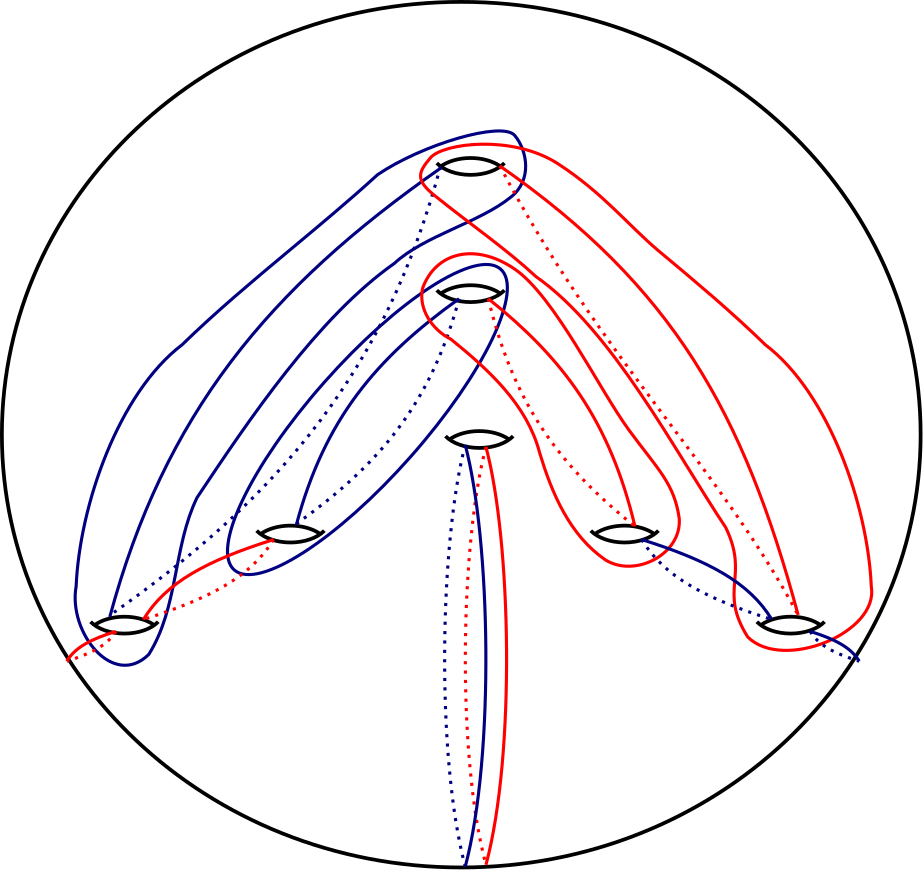
\includegraphics[height=3in]{diagrampart1.png}
\caption{The $\alpha$ and $\beta$ curves when $g=2$.}
\label{firsttwocolors}
\end{figure}

\begin{figure}[h]
\centering
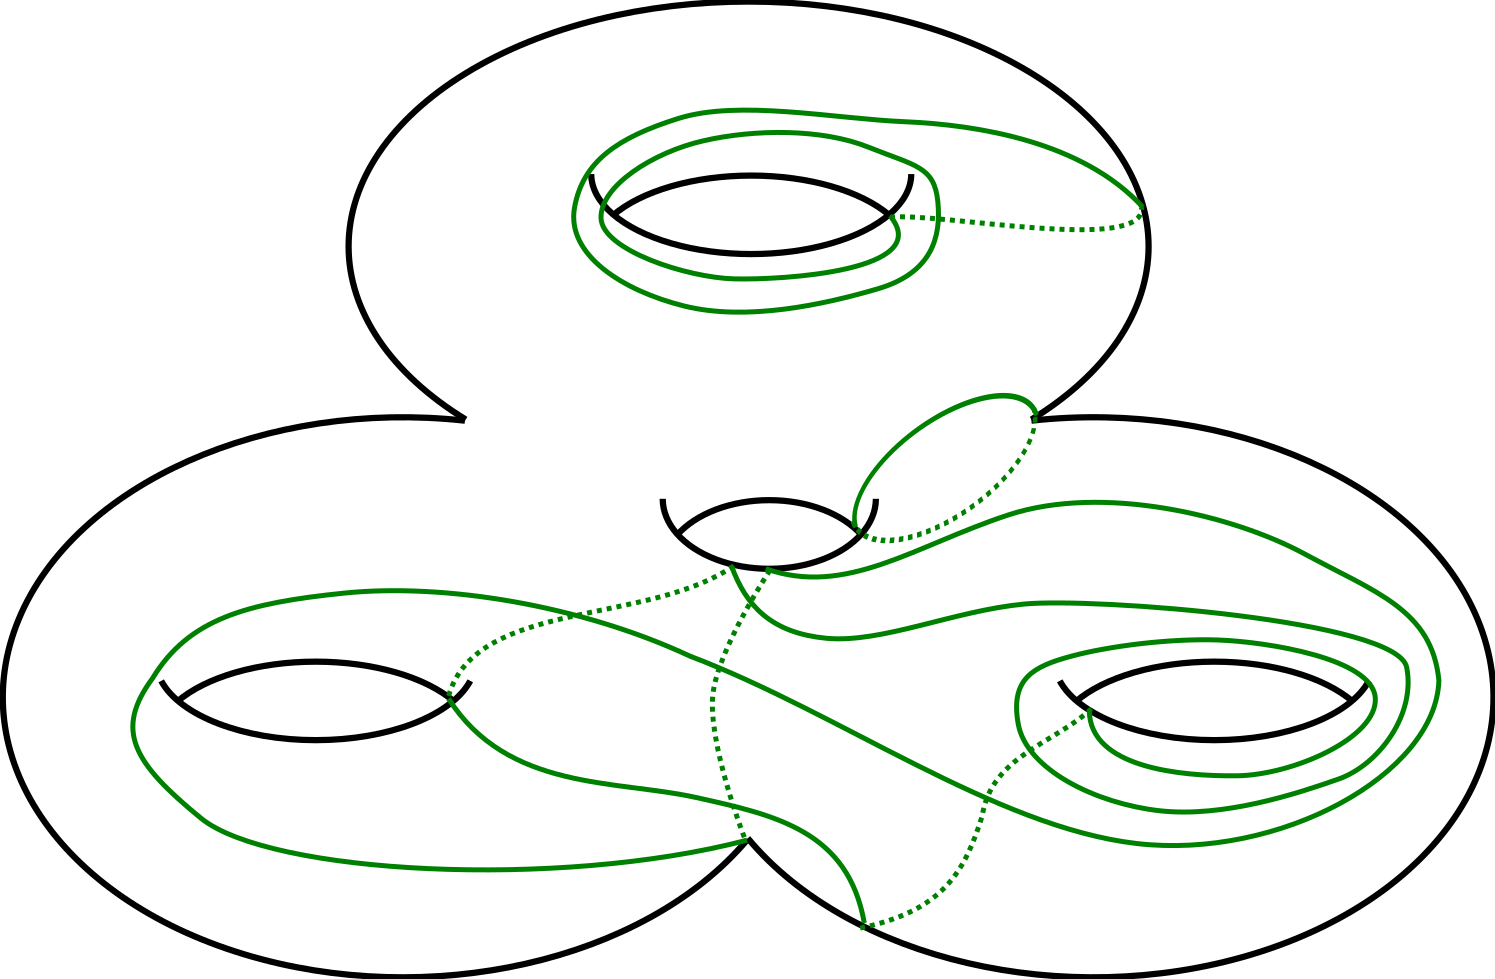
\includegraphics[height=3in]{s1rp3_green.png}
\caption{The set of $\gamma$ curves when $M =\R P^3$ and $\varphi$ flips $H_1$ and $H_2$.
Restricting the bottom two $\gamma$ curves to $\Sigma_3$ gives a pair of trivial looking arcs that turn into complicated arcs when $\eta_{3 \to 1}$ is applied to the surface.
Connecting the former arcs with the latter, keeping orientations of the arcs in mind, produces the full $\gamma$ curves.}
\label{greenex}
\end{figure}

\smallskip
\noindent\textit{Case 2: $\varphi$ preserves the Heegaard splitting}\ \

We begin by constructing the genus $4g+1$ unbalanced trisection shown in Figure \ref{unbalancedbreakdown} by attaching tubes through the areas indicated by horizontal lines as in the previous constructions.
After constructing a diagram for this trisection we will find a set of $g$ destabilizations resulting in a genus $3g+1$ diagram.
We conclude by showing that the destabilized trisection is the same as the trisection constructed in Section \ref{sec_mainthm}.

\begin{figure}[h]
\centering
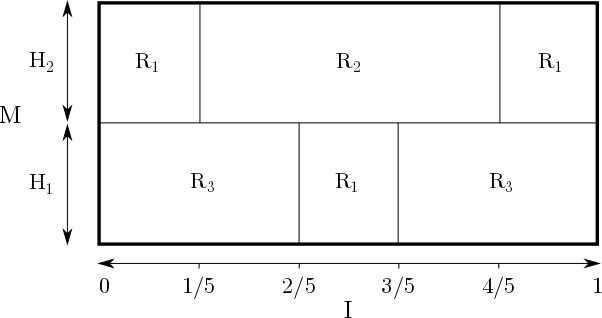
\includegraphics[height=1.8in]{MxS1_unbalanced.png}
\caption{$I \times M$ is depicted as a rectangle with $I$ as the horizontal axis and $M$ as the vertical axis.
The middle horizontal line represents $I \times \Sigma$, so the copy of $M$ represented by each vertical slice is cut by the middle line into copies of the handlebodies $H_1$ and $H_2$.}
\label{unbalancedbreakdown}
\end{figure}

To begin, draw the triple intersection surface for this diagram as four twice punctured copies of $\Sigma$ connected by tubes.
Call the four copies $\Sigma_1, \Sigma_2, \Sigma_3$, and $\Sigma_4$ where $\Sigma_i$ of cyclically adjacent indices are connected by tubes.
In our construction $\Sigma_1, \Sigma_2, \Sigma_3$, and $\Sigma_4$ correspond to the copies of $\Sigma$ lying in $M_{1/5}, M_{2/5}, M_{3/5}$, and $M_{4/5}$ respectively, and can be pictured as lying at the triple intersection corners in Figure \ref{preservebreakdown}.
Similar to the case where $\varphi$ flips the Heegaard splitting, $[1/5, 4/5] \times \Sigma \subset [1/5, 4/5] \times M$ induces identifications $\eta_{i \to j}\colon \Sigma_i \to \Sigma_j$ for all $1 \le i < j \le 4$.
$I_{13} \times M$ induces a different identification $\eta_{4 \to 1}\colon \Sigma_4 \to \Sigma_1$.
By the same argument as in the case of $\varphi$ flipping the Heegaard splitting, we see that $\eta_{4 \to 1} = (\eta_{1 \to 4}^{-1} \circ \varphi)$.

Draw the $\Sigma_i$ in the plane at evenly distributed $\theta$ values $\theta_1$, $\theta_2$, $\theta_3$, and $\theta_4$, with all holes of $\Sigma_i$ lying along the $\theta_i$ axis.
Reflect each of $\Sigma_2$ and $\Sigma_4$ locally in $\theta$ as we did with $\Sigma_2$ in the case where $\varphi$ flips the Heegaard splitting.
Thus, $\eta_{1 \to 3}$ is the result rotating $\Sigma_1$ around the center of the diagram from $\theta_1$ to $\theta_3$.
$\eta_{1 \to 2}$ (resp. $\eta_{1 \to 4}$) is the result of rotating $\Sigma_1$ from $\theta_1$ to $\theta_2$ (resp. $\theta_4$) and then reflecting.
This ensures that the curves bounding product disks in the copies of $I_{ij} \times (\Sigma - D^2)$ are symmetric except for the curves bounding disks in $I_{13} \times (\Sigma - D^2)$.
In the case of $I_{13} \times (\Sigma - D^2)$, given an essential arc $c$ in $\Sigma - D^2$, the disk $I_{13} \times c$ has boundary consisting of $c \subset \Sigma_4 - D^2$, $\eta_{4 \to 1}(c) \subset \Sigma_1 - D^2$, and two arcs in the tube between $\Sigma_1$ and $\Sigma_4$ connecting $c$ with $\eta_{4 \to 1}(c)$.
The two arcs connect $c$ with its image with the opposite orientation, so an endpoint of $c$ is connected up to the image under $\eta_{4 \to 1}$ of the same endpoint in $\eta_{4 \to 1}(c)$.

Again let $\theta_{ij}$ be the angle halfway between $\theta_i$ and $\theta_j$, lying in the smaller ($< \pi$) angular region between them.
The algorithm to draw the diagram on this surface is then:

\begin{enumerate}
\item Draw the genus $4g+1$ surface as copies of $\Sigma_i$, $i = 1,2,3,4$ with surfaces at adjacent indices connected by tubes.
\item Draw $2g$ nonseparating disjoint $\gamma$ curves symmetric about $\theta_{12}$ and avoiding $\Sigma_3$ and $\Sigma_4$, and another $2g$ $\gamma$ curves symmetric about $\theta_{34}$ and avoiding $\Sigma_1$ and $\Sigma_2$.
\item Draw a single $\gamma$ curve as a meridian of the tube connecting $\Sigma_1$ and $\Sigma_4$.
\item Draw $2g$ nonseparating disjoint $\alpha$ curves symmetric about $\theta_{23}$ and avoiding $\Sigma_1$ and $\Sigma_4$.
\item Draw a single $\beta$ and $\gamma$ curve each around either the tube connecting $\Sigma_1$ and $\Sigma_2$ or the tube connecting $\Sigma_3$ and $\Sigma_4$.
The two choices are slide equivalent.
\item Draw a cut system for $H_2$ consisting of $\alpha$ curves on $\Sigma_1$.
\item Draw a reflected cut system for $H_2$ consisting of $\alpha$ curves on $\Sigma_4$.
\item Draw a cut system for $H_1$ on each of $\Sigma_2$ and $\Sigma_3$ consisting of $\beta$ curves.
\item Let $c_1,\cdots,c_{2g}$ be a nonseparating collection of disjoint arcs in $\Sigma_4$ with their boundaries lying on the puncture of $\Sigma_4$ that is tubed to $\Sigma_1$.
Then connect each $c_i$ to its image $\eta_{4 \to 1}(c_i)$ in $\Sigma_1$ with the opposite orientation.
Draw these $2g$ curves as $\beta$ curves.
Note that the $\eta_{4 \to 1}(c_i)$ will need to be drawn reflected in $\theta$ because $\eta_{1 \to 4}$ reflected the embedding of $\Sigma_4$ relative to $\Sigma_1$.
If $\eta_{4 \to 1}$ acts trivially on $\Sigma$ these curves will look symmetric about $\theta_{41}$.
\end{enumerate}

An example is shown in Figure \ref{unbalancedex}.



\begin{figure}[h]
\centering
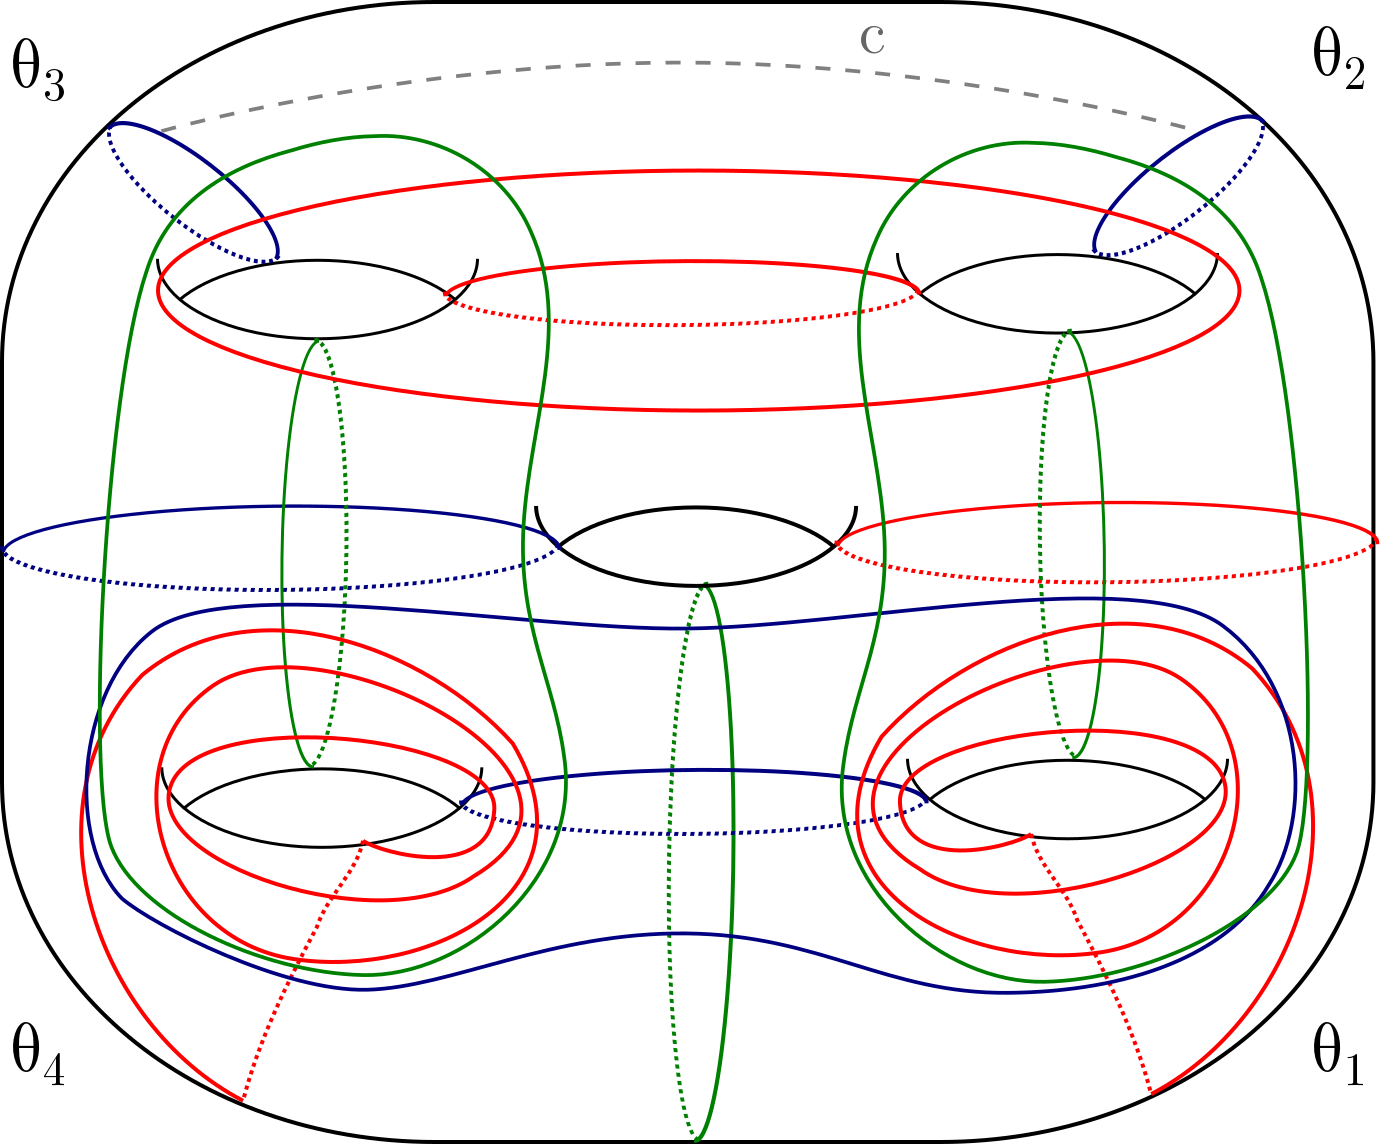
\includegraphics[height=3in]{LxS12.png}
\caption{A diagram for the genus $5$ trisection where $M = L(3,1)$ and $\varphi$ is the identity.
}
\label{unbalancedex}
\end{figure}

We now show that this diagram can always be destabilized $g$ times.
First, choose the symmetric $\alpha$ and $\gamma$ curves from steps (2) and (4) to consist of curves that either look like meridians in the chosen embedding or that lie on the near side of the surface in the diagram (in the sense that we can draw it on the diagram using a solid line) and loop around one of those meridians, as in Figure \ref{unbalancedex}.
Next, slide the $\beta$ meridian curves lying on $\Sigma_3$ to be parallel to the $g$ $\alpha$ curves that look like meridians symmetric across $\theta_{23}$.
In Figure \ref{unbalancedex}, this slide is guided by the path $c$.
At this point we have $g$ pairs of parallel $\alpha$ and $\beta$ curves, and the isotopy class of this curve intersects two of the $\gamma$ curves in one point each.
See Figure \ref{destabpartial} for a partial trisection diagram in the case where $g=2$.
The $\alpha$ and $\beta$ curves depending on the monodromy or Heegaard diagram have not been drawn, so the partial diagram of Figure \ref{destabpartial} is actually general for the case where $g=2$.

For each pair, we can slide one of these $\gamma$ curves over the other, after which we have a parallel $\alpha$ and $\beta$ curve that each intersect the set of $\gamma$ curves in a single point.
This implies that our diagram is a ($g$ times) unbalanced stabilization, and the destabilization can be achieved by compressing the surface along the isotopy classes of each parallel $\alpha$ and $\beta$ curves, deleting the now trivial $\alpha$ and $\beta$ curves together with the $\gamma$ curve that they intersect.
See Figure \ref{ls12destab} for the diagram resulting from destabilizing the trisection in Figure \ref{unbalancedex}.


\begin{figure}[h]
\centering
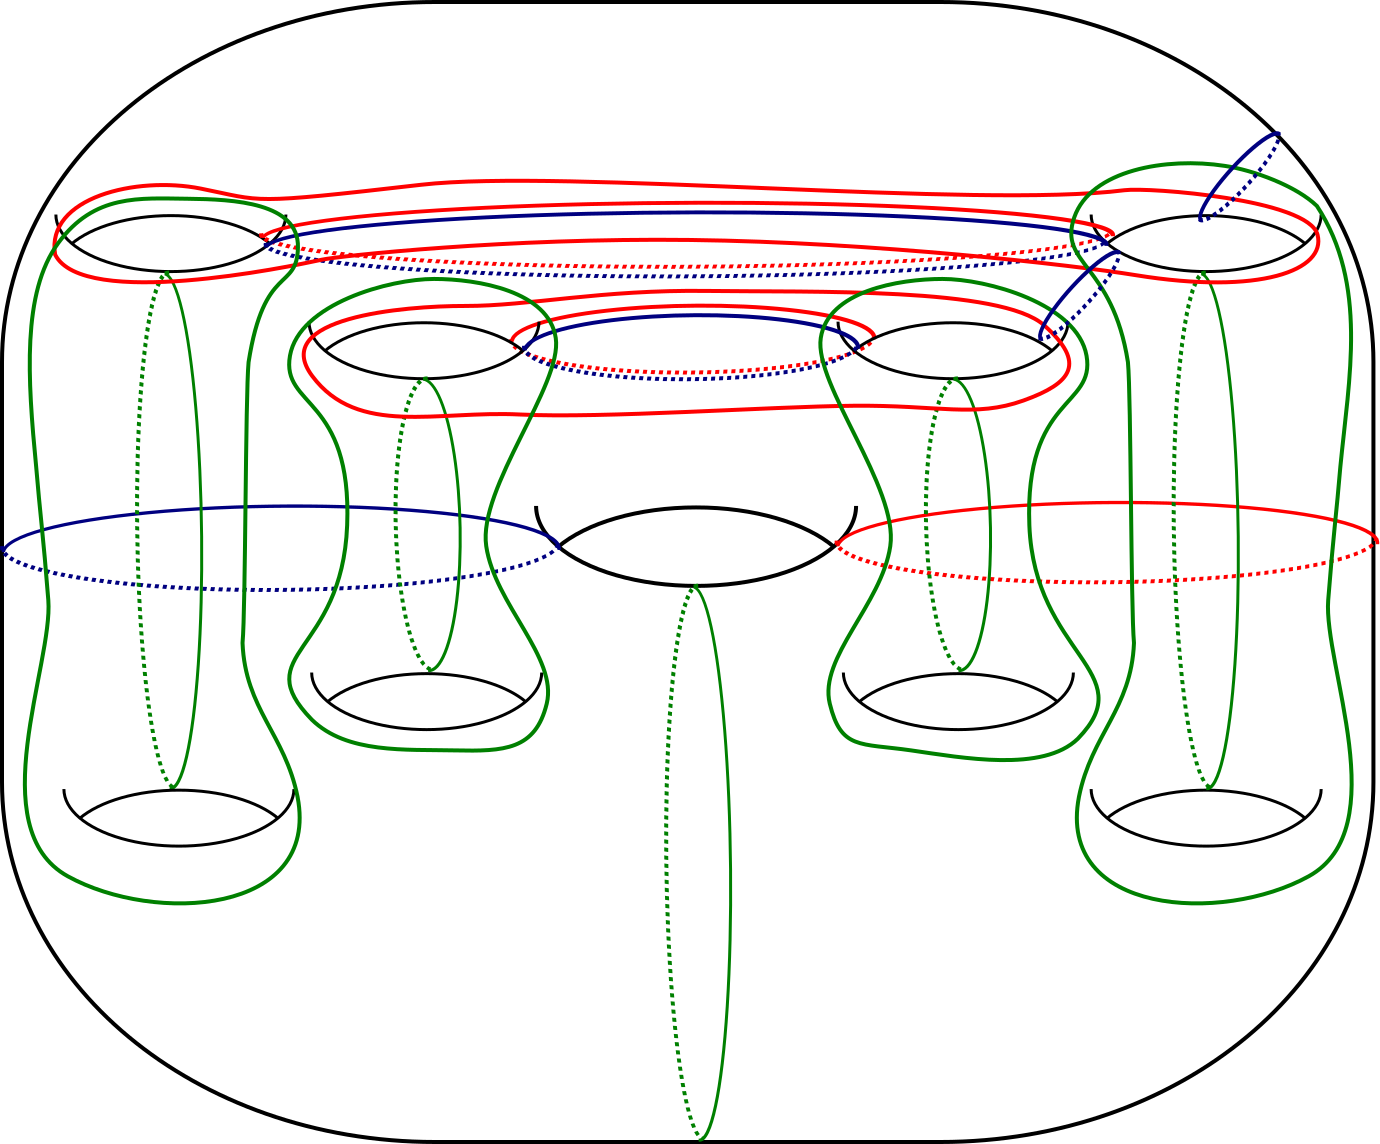
\includegraphics[height=3in]{finddestabpartial.png}
\caption{A partial trisection diagram for for finding destabilizations in the case where $g=2$.
Note that additional curves that would be required to complete the diagram will not interfere with the destabilizations.}
\label{destabpartial}
\end{figure}

\begin{figure}[h]
\centering
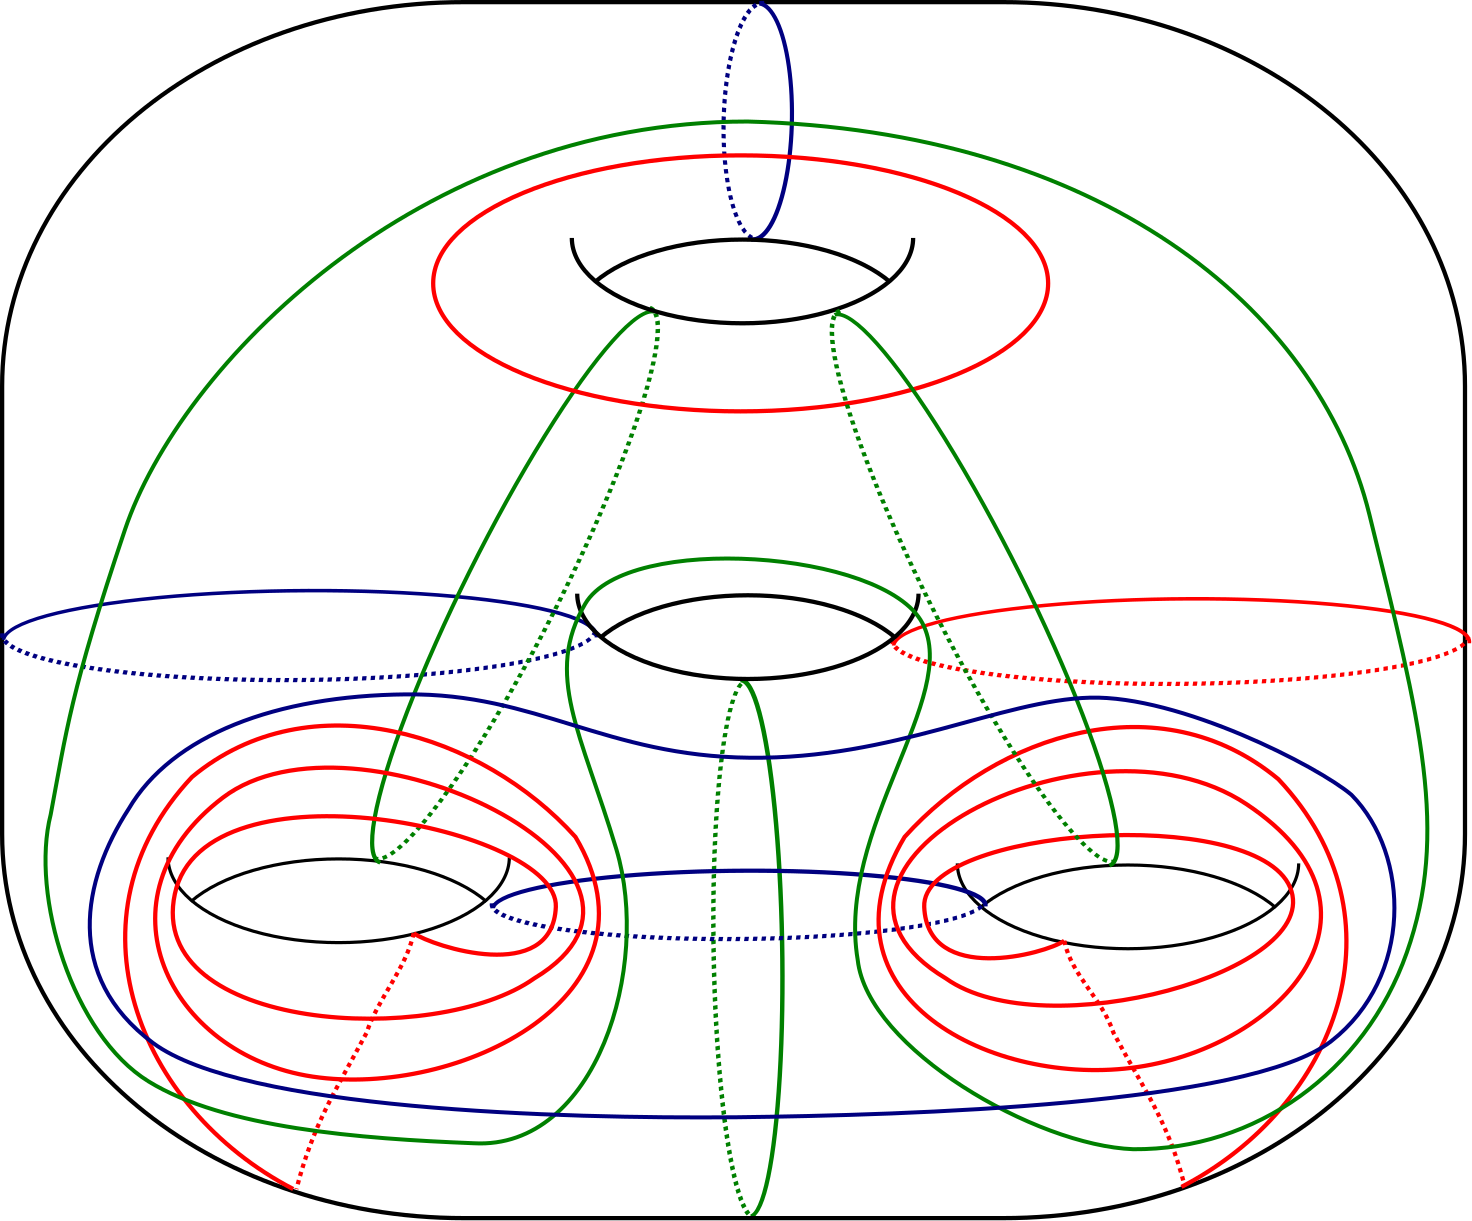
\includegraphics[height=3in]{LxS12destab.png}
\caption{A diagram for the genus 4 trisection where $M = L(3,1)$ and $\varphi$ is the identity.
}
\label{ls12destab}
\end{figure}

Although the above argument is sufficient to prove that $X$ has a genus $3g+1$ trisection diagram, we have yet shown that the diagram gives the same trisection as the one constructed in the main theorem.
We analyze how these destabilizations affect the trisection itself to show that these destabilizations actually do produce the genus $3g+1$ trisection constructed earlier.


Each destabilization is given by a parallel $\alpha$ and $\beta$ curve, both dual to a single $\gamma$ curve.
Reindex to denote the sets of three curves by $\alpha_i,\beta_i$ and $\gamma_i$ for $1 \le i \le g$.
Suppose $D_{\alpha_i}$ be a meridian disk of $X_1 \cap X_2$ with boundary $\alpha_i$, and $D_{\beta_i}$ a meridian disk of $X_1 \cap X_3$ with boundary $\beta_i$.
Then $D_{\alpha_i} \cup D_{\beta_i}$ is a 2--sphere lying in $\del X_1$, and therefore bounds a 3--ball $B_i$ in $X_1$ by \cite{LaudenbachPoenaru1}.
Hence each $D_{\alpha_i} \cup D_{\beta_i}$ is the belt sphere of a 1--handle in a handle decomposition of $X_1$.
The destabilizations are therefore obtained by ``compressing'' $X_1$ along $B_i$.
If $N(B_i)$ is a regular neighborhood of $B_i$ in $X_1$, we replace $X_1$ with $X_1 - N(B_i)$ and replace $X_2$ with $X_2 \cup N(B_i)$ (choosing $X_3$ instead of $X_2$ here is topologically equivalent).
Each compression decreases the genus of $X_1$ by 1.  We will find destabilizations by defining such pairs of disks $D_{\alpha_i}$ and $D_{\beta_i}$.

Let $x \in \mathring I_{12}$ and look at a single slice $M_x = \{x\} \times M$.
Then $M_x \cap X_1 = H_1 - B_{12}$, $M_x \cap X_2 = H_2 - B_{12}$, and $M_x \cap X_3 = B_{12}$.
$M_x \cap \alpha_i = M_x \cap \beta_i$ is a pair of two points.
We can connect these two points with an arc of $D_{\alpha_i}$ in $(H_1 - B_{12}) \cap H_2 = M_x \cap X_1 \cap X_2$ and an arc of $D_{\beta_i}$ in $B_{12} \cap (H_1 - B_{12}) = M_x \cap X_1 \cap X_3$.
In this way, we can obtain disks $D_{\alpha_i}$ and $D_{\beta_i}$ bounded by $\alpha_i = \beta_i$ by taking the union of these arcs for all $x \in I_{12}$.
The disks $D_{\alpha_i}$ and $D_{\beta_i}$ are each capped off on the two sides by an arc of the intersection of $\alpha_i = \beta_i$ with $\Sigma_2 \subset M_{2/5}$ and an arc of the intersection with $\Sigma_3 \subset M_{3/5}$.

We now need to find the ball $B_i \subset X_1$ bounded by $D_{\alpha_i} \cup D_{\alpha_i}$.
Looking back at a single $M_x$, the union of the arc from $D_{\alpha_i}$ and the arc from $D_{\beta_i}$ is a simple closed curve in $\del (H_1 - B_{12})$, and this curve bounds a disk $D_i$ in $H_1 - B_{12}$.
See Figure \ref{getU}.
It follows that the ball $B_i$ is in fact $I_{12} \times D_i$, so the destabilization is achieved by setting

\begin{align*}
&X_1' = X_1 - N(I_{12} \times D_i) \\
&X_2' = X_2\\
&X_3' = X_3 \cup N(I_{12} \times D_i)
\end{align*}

\begin{figure}[h]
\centering
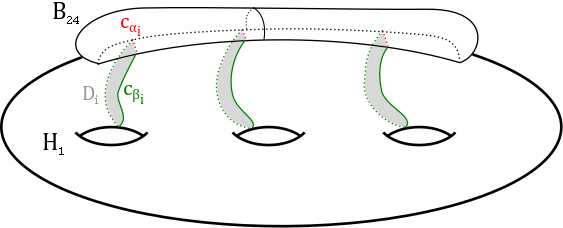
\includegraphics[height=1.8in]{gettingU.png}
\caption{In a given slice $M_x$ we see disks $D_i$ coming from the intersections $M_x \cap B_i$, where each $B_i$ is a 3--ball giving a destabilization.
Note that the complement of the disks $D_i$ in $H_1$ is also a topological ball.
}
\label{getU}
\end{figure}

Note that moving $\bigcup_{i=1}^g N(I_{12} \times D_i)$ to the $X_2'$ region rather than the $X_3'$ region would give the same topological result.

There are $g$ such destabilizations, so to get the final result we must find disjoint $D_1 \cdots D_g$ such that $B_i = I_{12} \times D_i$, and setting
\begin{align*}
&X_1' = X_1 - \bigcup_{i=1}^g N(I_{12} \times D_i) \\
&X_2' = X_2\\
&X_3' = X_3 \cup \bigcup_{i=1}^g N(I_{12} \times D_i)
\end{align*}

In the result of destabilization, $X_3' \cap M_x = B_{12} \cup \bigcup_{i=1}^g N(I_{12} \times D_i)$.
This is a topological ball as can be seen in Figure \ref{getU} (the union of $B_{12}$ and regular neighborhoods of the disks in the figure).
$X_1' \cap M_x$ consists of the complement of the disks $D_i$ in $H_1$, so it is also a topological ball.  
We can then set  $U=X_1' \cap M_x$ and $V = X_3' \cap M_x$.  The boundary $U \cap V$ consists of four disks, two of which are shown in Figure \ref{fig_uvboundary}.  Figure \ref{fig_splittinguv} shows that by performing an isotopy, we can in fact achieve the same split $U \cap V$ as in Figure \ref{fig_disjointballs}.
Thus, we have obtained the same genus $3g+1$ trisection as constructed in Section \ref{sec_mainthm}.

\begin{figure}[h]
\centering
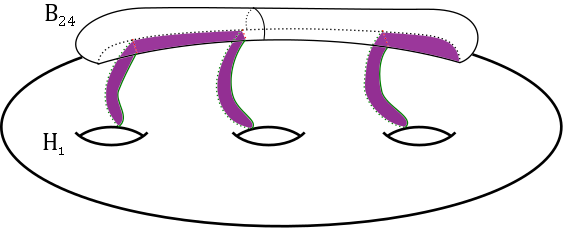
\includegraphics[height=1.6in]{UVboundary.png}
\caption{Two of four disks of the intersection $U \cap V$ are shown in purple.
}
\label{fig_uvboundary}
\end{figure}

\begin{figure}[h]
\centering
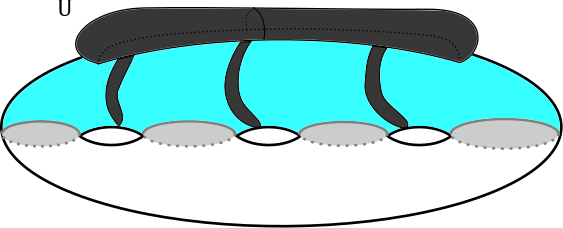
\includegraphics[height=1.6in]{splittingUV.png}
\caption{Each of the four teal regions is a topological ball meeting the dark region $U$ in a disk.  Thus, $U$ can be isotoped to the union of the dark and teal regions.
}
\label{fig_splittinguv}
\end{figure}

%%%%%%%%%

\section{Further Questions}
\label{sec_questions}

We end by leaving a few unanswered questions for the interested reader.

\begin{question}
Is there some choice of $M$ and $\varphi$ such that there exists a trisection of genus lower than $3g+1$, where $g$ is the minimal genus of a Heegard splitting of $M$?
\end{question}

We next ask if we get the same in cases where we could apply both methods to get two trisections of $X$.

\begin{question}
Suppose that $\varphi$ can be chosen up to composition with an isotopy to either preserve or flip a Heegaard splitting of $M$.
 Are the trisections produced in these two cases equivalent?
\label{unequal1}
\end{question}

The above question might be easier to approach by first assuming $X$ is a product manifold $S^1 \times M$ where $M$ has a flippable Heegaard splitting.


We note that the construction in the case where $\varphi$ preserves the Heegaard splitting creates the trisection in an assymmetric manner, where the $X_i$ play different roles.
This leads to the following questions:
\begin{question}
\label{q_assym}
Is there a more symmetric construction of a $(3g+1;g+1)$--trisection in the case where $\varphi$ preserves the Heegaard splitting?  Is there a symmetric or nearly symmetric diagram?
\end{question}

\begin{question}
Suppose $\varphi$ preserves the Heegaard splitting and we use the methods of this paper to construct a $(3g+1;g+1)$--trisection.
Does rotating the indices of the $X_i$ always produce an equivalent trisection?
\label{unequal3}
\end{question}

Baykur and Saeki found genus $3g+1$ trisections in the case of Heegaard splitting preserving monodromy using simplified broken Lefschetz fibrations \cite{BaykurSaeki1}.
Their methods give a trisection map $X \to D^2$ with symmetric singular set, providing a partial answer to question \ref{q_assym}.
However, it is difficult to obtain diagrams from their construction or to analyze precisely how the trisections cut up the manifold.


A fundamental question in trisection theory is that of analyzing when a 4--manifold has multiple nonequivalent trisections of the same genus.
Gabriel Islambouli has produced a class of examples relying on distinguishing the Nielsen classes of the fundamental group generators coming from the spines of the $X_i$ \cite{Islambouli1}.
The results build off of similar results on Heegaard splittings, using classes of 3--manifolds with multiple distinct Heegaard splittings of the same genus.
An answer of ``no" to one of questions \ref{unequal1} or \ref{unequal3} would provide new examples, possibly even in the case where $M$ has a unique genus $g$ Heegaard splitting.


\bibliographystyle{amsplain}
\bibliography{Trisections}{}


% --------------------------------------------------------------
%
% --------------------------------------------------------------

% --------------------------------------------------------------
%
% --------------------------------------------------------------

\end{document}
